\FloatBarrier
\section{Tecnologia, calibração e solução contínua}\label{app:calibration_details}\label{app:derivations}
\subsection{Horas físicas e trabalho efetivo}\label{app:kappa_deriv}
Para o grupo $g$, sejam $\theta_{gb}$ os pesos da distribuição formal e $h_{gb}$ as horas habituais observadas. O estado inicial principal usa $H_0=44$ e $h_{gb}^0=\min\{h_{gb},44\}$; a distribuição integral é sensibilidade. Defina
\begin{align}
\bar h_{F,g}(H)&=\sum_b\theta_{gb}\min\{h_{gb},H\},\\
q_{F,g}(H)&=\sum_b\theta_{gb}\min\{h_{gb},H\}\,e\!\left(\min\{h_{gb},H\}\right),\qquad q_{I,g}=h_{I,g}e(h_{I,g}).\label{eq:app_effective_hours}
\end{align}
Horas efetivas na pesquisa e trabalho efetivo no modelo são distintos: o segundo multiplica horas físicas por eficiência tecnológica. Não se substitui a média de $he(h)$ pelo produto de médias independentes. As funções comparadas são
\begin{equation}\label{eq:app_efficiency}
e_B(h)=\exp\{-\kappa(h-h^*)^2\},\qquad e_F(h)=\exp\{-\kappa[\max\{h-h^*,0\}]^2\}.
\end{equation}
Coincidem para $h\geq h^*$; abaixo do pico, a primeira penaliza desvios e a segunda mantém eficiência unitária. O pico é da eficiência por hora, não necessariamente do produto. Como o estado inicial contém jornadas abaixo do pico e a ponte é recalibrada por função, essa coincidência não implica curvas de $\Areq$ exatamente iguais em tetos acima dele.

A elasticidade que ancora a curvatura é a de $q(h)=he(h)$:
\begin{equation}\label{eq:kappa_derivation}
\varepsilon_q=\left.\frac{d\log q(h)}{d\log h}\right|_{h=h_{\mathrm{ref}}}=1-2\kappa h_{\mathrm{ref}}(h_{\mathrm{ref}}-h^*),\quad
\kappa=\frac{1-\varepsilon_q}{2h_{\mathrm{ref}}(h_{\mathrm{ref}}-h^*)}.
\end{equation}
Na função de fadiga, exige-se $h_{\mathrm{ref}}>h^*$. Abaixo do pico, a elasticidade é um e não identifica $\kappa$. Mantêm-se as hipóteses externas $h_{\mathrm{ref}}=42{,}244$, $h^*=40$ e $\varepsilon_q=0{,}6$, resultando em $\kappa=0{,}002109804$. A referência não é a nova média PNAD. Separá-la da distribuição evita alterar silenciosamente a hipótese de eficiência. Com $\varepsilon_q=1$, impõe-se $\kappa=0$.

A literatura de horas longas motiva testar rendimentos decrescentes, mas não identifica esses parâmetros para o Brasil nem a penalidade bilateral em jornadas curtas \citep{Pencavel2015,CollewetSauermann2017}. A extrapolação à cauda longa é substantiva, como mostra a Seção~\ref{app:hours_efficiency}. $\varepsilon_q$ não é a elasticidade do produto agregado em relação às horas, que depende também da composição e dos agregadores.

\subsection{Produção, objetivo e fronteiras}
Cada grupo produz com capital fixo:
\begin{align}
Y_g&=A_gK_g^\alpha L_g^{1-\alpha},\qquad L_g=\left[\omega_g L_{F,g}^{\rho}+(1-\omega_g)L_{I,g}^{\rho}\right]^{1/\rho},\label{eq:app_production}\\
L_{F,g}&=N_{F,g}q_{F,g},\quad L_{I,g}=\eta_I N_{I,g}q_{I,g},\quad \rho=\frac{\sigma-1}{\sigma},\quad N_{I,g}=N_g-N_{F,g}.
\end{align}
O limite $\sigma=1$ é Cobb--Douglas. Para $0<\omega_g<1$ e insumos positivos, os produtos marginais por trabalhador adicional, mantendo a outra modalidade fixa, são
\begin{align}
\mathrm{MP}_{F,g}&=(1-\alpha)Y_gL_g^{-\rho}\omega_gL_{F,g}^{\rho-1}q_{F,g},\label{eq:app_mpf}\\
\mathrm{MP}_{I,g}&=(1-\alpha)Y_gL_g^{-\rho}(1-\omega_g)L_{I,g}^{\rho-1}\eta_Iq_{I,g}.\label{eq:app_mpi}
\end{align}
Têm unidades de produto semanal por trabalhador; os marginais por unidade de trabalho efetivo são outros objetos. A escolha privada contínua é
\begin{equation}\label{eq:app_objective}
\max_{0\leq x\leq N_g}J_g(x)=Y_g(x,N_g-x)-\tau_gx-\frac{\pi_g}{2}(N_g-x)^2-\frac{\gamma_g}{2}(x-\bar N_{F,g})^2.
\end{equation}
Sua condição interior é
\begin{equation}\label{eq:foc_NF}
J'_g(x)=\mathrm{MP}_{F,g}-\mathrm{MP}_{I,g}-\tau_g+\pi_g(N_g-x)-\gamma_g(x-\bar N_{F,g})=0.
\end{equation}
A diferença dos marginais é necessária porque uma unidade formal adicional retira uma informal. O termo positivo de $\pi_gN_{I,g}$ é a redução de custo informal. Não se multiplica novamente pela derivada CES após calcular $\mathrm{MP}_{F,g}$.

Para $\sigma>0$, $0<\alpha<1$, capital positivo e custos convexos não negativos, a produção composta é côncava na composição. As condições interiores e de fronteira caracterizam o máximo global. Em $x=0$, exige-se $J'_g(0^+)\leq0$; em $x=N_g$, $J'_g(N_g^-)\geq0$. O algoritmo usa limites direcionais da tecnologia, resolve a raiz interior por Brent e compara objetivos nos extremos. Proximidade numérica de um extremo não certifica otimalidade sem essas condições. Registram-se resíduo da derivada, violação de otimalidade e posição interior ou de fronteira.

\subsection{Normalização das cunhas}
O alvo de informalidade determina $\bar N_{F,g}=(1-i_g)N_g$ e $\bar N_{I,g}=i_gN_g$. No estado inicial, o custo de ajuste tem derivada zero. Com $D_g=\mathrm{MP}_{F,g}^0-\mathrm{MP}_{I,g}^0$, o momento identifica apenas
\begin{equation}\label{eq:app_wedge_identification}
\tau_g-\pi_g\bar N_{I,g}=D_g.
\end{equation}
Seleciona-se uma solução não negativa por normalização:
\begin{equation}\label{eq:app_wedge_normalization}
\tau_g\geq0,\quad\pi_g\geq0,\quad\tau_g\pi_g=0,\qquad
(\tau_g,\pi_g)=\begin{cases}(D_g,0),&D_g\geq0,\\(0,-D_g/\bar N_{I,g}),&D_g<0.\end{cases}
\end{equation}
A complementaridade separa coeficientes por convenção, sem identificação independente. Cada mudança de tecnologia ou distribuição exige recalibrar o par. Seus valores dependem das normalizações e não são alíquotas de folha ou estimativas de fiscalização. No cenário principal, $\tau_B=2{,}661015$ e $\tau_F=2{,}714237$, com $\pi=0$. Mantém-se $\gamma=0{,}06$ como hipótese.

\subsection{Ponte formal--informal e identificação condicional}\label{app:sigma_discussion}
As elasticidades de substituição dependem dos tipos de trabalho e da margem modelada. \citet{OttavianoPeri2012} estudam substituição entre nativos e imigrantes; \citet{BaharDiTellaGulek2025} examinam choques de oferta informal e permissões de trabalho. Aqui, $\sigma_{\mathrm{sub}}$ governa a substituição entre trabalho efetivo formal e informal no agregador de produção. \citet{LeyvaUrrutia2020} incorporam fricções de emprego e participação, enquanto \citet{McKiernan2021} considera a alocação de tempo das famílias entre trabalho formal, informal e produção doméstica. Essas diferenças de objeto e de estrutura impedem transportar diretamente as elasticidades entre modelos.

Mantém-se $\sigma=1{,}326$, calibrando $\omega$ condicionalmente à razão horária da Equação~\eqref{eq:app_observed_bridge}, com horas formais limitadas a 44h no alvo principal. Participação formal no emprego ou na renda não é, por identidade, peso tecnológico CES. Definindo $P_F=\sum_gN_{F,g}\mathrm{MP}_{F,g}$ e $P_I=\sum_gN_{I,g}\mathrm{MP}_{I,g}$, a ponte é
\begin{align}
R_h^{\mathrm{modelo}}&=\frac{P_F/\sum_gN_{F,g}\bar h_{F,g}}{P_I/\sum_gN_{I,g}h_{I,g}},\label{eq:app_model_bridge}\\
R_w^{\mathrm{modelo}}&=\frac{P_F/\sum_gN_{F,g}}{P_I/\sum_gN_{I,g}}.
\end{align}
Marginais são calculados por grupo antes de agregar folhas e horas. Um CES dos insumos somados não reproduz, em geral, essa agregação. A identidade $N_{F,g}\mathrm{MP}_{F,g}+N_{I,g}\mathrm{MP}_{I,g}=(1-\alpha)Y_g$ é controle de implementação.

Igualar marginais brutos a remunerações acrescenta hipótese competitiva ao problema privado com $N_g$ fixo. Esse problema isoladamente não determina salários líquidos ou distribuição de transferências. $R_h^{44}=1{,}682473$ gera $\omega_B=0{,}675651$ e $\omega_F=0{,}676650$. A razão semanal é $1{,}894029$ no modelo e $1{,}880100$ na amostra paga; o desvio $0{,}013929$ é reportado, pois ela não foi o alvo. Sua relação com as mesmas folhas e horas, além das diferenças de universo, impede interpretar proximidade como validação independente.

Uma razão não identifica conjuntamente $\sigma$, $\omega$, $\eta_I$ e cunhas. $\eta_I=0{,}40$ é hipótese de eficiência, não razão de rendimentos. Na mensuração das participações dos fatores, \citet{Gollin2002} mostra que omitir a remuneração do trabalho dos autônomos subestima a parcela do trabalho. Seus rendimentos combinam trabalho e capital. Aqui, $\alpha=0{,}35$ permanece uma hipótese, sem nova estimação dessa parcela.

\FloatBarrier
\section{Restauração do produto e recursos}\label{app:areq_resources}
\subsection{Composição reotimizada e congelada}
Para um multiplicador comum $a>0$, cada grupo resolve novamente a Equação~\eqref{eq:app_objective}, com $aA_g$. A compensação satisfaz
\begin{equation}\label{eq:app_areq}
\sum_gY_g\big(aA_g,H,N_{F,g}^*(a,H)\big)=Y_0,\qquad \Areq=a-1.
\end{equation}
A compensação é uma fração; sua expressão em porcentagem nas tabelas é $100\Areq$. A reotimização ocorre em cada avaliação da raiz e já existia no algoritmo original. O núcleo comum a preserva, verifica o intervalo da raiz e o amplia quando necessário. O erro relativo de restauração deve ser menor que $10^{-9}$.

A monotonicidade relevante é a da produção escolhida, não a de cada emprego ou insumo. Escreva a produção como $af_g(x)$ e os custos como $c_g(x)$. Se $x_1,x_2$ maximizam o objetivo em $a_1<a_2$, preferência revelada fornece
\begin{align*}
a_1f_g(x_1)-c_g(x_1)&\geq a_1f_g(x_2)-c_g(x_2),\\
a_2f_g(x_2)-c_g(x_2)&\geq a_2f_g(x_1)-c_g(x_1).
\end{align*}
Somando, $(a_2-a_1)[f_g(x_2)-f_g(x_1)]\geq0$. Portanto, $af_g(x^*(a))$ cresce estritamente onde a produção é positiva, mesmo sem monotonicidade da composição formal. Isso sustenta a raiz com custos e parâmetros fixos durante a busca.

A compensação congelada fixa o emprego no valor efetivamente obtido no estado inicial. Pela linearidade em $a$,
\begin{equation}\label{eq:app_areq_frozen}
\Areq^{\mathrm{fixa}}=\frac{Y_0}{\sum_gY_g(A_g,H,N_{F,g}^0)}-1.
\end{equation}
\begingroup\widowpenalty=10000\clubpenalty=10000
Ela não congela horas ou eficiência. Para 36h, é $7{,}955504\%$ (bilateral) e $6{,}194459\%$ (fadiga), contra $8{,}381261\%$ e $6{,}524416\%$ reotimizados. Para 40h, é $1{,}494072\%$ e $1{,}457202\%$, contra $1{,}572576\%$ e $1{,}533765\%$.
\par\endgroup

$\Areq$ tem sinal. Se a intervenção já eleva produto, reduzi-lo ao inicial pode exigir queda de $A$, gerando raiz negativa. A necessidade de ganho adicional não negativo é $\max\{\Areq,0\}$. Ambas as compensações se referem ao produto bruto, não ao consumo líquido.

\subsection{Pagamentos e fechamento}\label{app:pe_omits}
No fechamento principal, $\tau_gN_{F,g}$ e $\pi_gN_{I,g}^2/2$ são pagamentos privados devolvidos ao domicílio. O ajuste $D_g^{\mathrm{aj}}=\gamma_g(N_{F,g}-\bar N_{F,g})^2/2$ consome recursos:
\begin{equation}\label{eq:app_resources}
C^{\mathrm{ag}}+\sum_gD_g^{\mathrm{aj}}=\sum_gY_g.
\end{equation}
A opção alternativa do código destrói também os demais pagamentos:
\begin{equation}\label{eq:app_resources_alternative}
C^{\mathrm{ag}}+\sum_g\left[D_g^{\mathrm{aj}}+\tau_gN_{F,g}+\frac{\pi_g}{2}N_{I,g}^2\right]=\sum_gY_g.
\end{equation}
A mudança afeta consumo e bem-estar, sem modificar a escolha privada se seu objetivo for mantido. Não se somam transferências a custos de recursos silenciosamente.

Capital e emprego total são fixos, nacionalmente e por setor. Ficam fora do exercício a acumulação de capital, os ajustes de salários e preços, a participação na força de trabalho, a acomodação monetária e fiscal e a realocação entre setores. A partilha de trabalho é desligada pela hipótese de $N$ fixo. Não há equações de investimento, barganha ou insumo-produto. O modelo não calcula ajuste de capital em três a cinco anos nem redução numérica de $\Areq$ por esse canal. Esses mecanismos não recebem sinal ou magnitude quantitativa; omiti-los tampouco demonstra que $\Areq$ seja limite superior. Sequências de tetos são comparações estáticas ao mesmo estado inicial, não trajetórias com aprendizado ou acumulação.

\FloatBarrier
\section{Bem-estar representativo e equivalente de consumo}\label{app:welfare_additional}
Sejam $c=C^{\mathrm{ag}}/N$ o consumo por trabalhador e $h$ a média de horas físicas, ponderando emprego formal e informal. O composto GHH é
\begin{equation}\label{eq:app_ghh}
G(c,h)=c-v(h),\qquad v(h)=\frac{\psi h^{1+\nu}}{1+\nu}.
\end{equation}
Usa-se $\nu=2$ e normaliza-se $\psi$ por $\psi h_0^\nu=w_0$, com $w_0=\sum_g(1-\alpha)Y_g^0/\sum_gN_gh_g^0$ imputado pela parcela do trabalho. É uma normalização representativa, não estimativa da desutilidade na PNAD. Publicam-se
\begin{align}
\Delta GHH\;(\%)&=100\frac{G(c_1,h_1)-G(c_0,h_0)}{G(c_0,h_0)},\label{eq:app_dghh}\\
CE\;(\%)&=100\frac{c_1-c_0-v(h_1)+v(h_0)}{c_0}.\label{eq:app_ce}
\end{align}
CE satisfaz $G(c_0[1+CE/100],h_0)=G(c_1,h_1)$. Numeradores iguais com denominadores distintos não são estatísticas intercambiáveis. Denominadores inválidos são tratados como erro, não substituídos por valores arbitrários.

Em 40h, o cenário principal dá $\Delta GHH=0{,}2250\%$ e $CE=0{,}1762\%$ na bilateral; na fadiga, $0{,}2763\%$ e $0{,}2164\%$. Em 36h, a bilateral dá $-4{,}3659\%$ e $-3{,}4199\%$, e a fadiga $-2{,}1210\%$ e $-1{,}6614\%$. São resultados sem compensação de produtividade, relativamente à base formal limitada a 44h. Restaurar produto e avaliar bem-estar diferem porque horas afetam desutilidade e custos consomem recursos.

Aplica-se $v$ à média de horas, não se calcula a média de $v(h_i)$ entre pessoas heterogêneas. Não há rendas individuais, transições identificadas ou regras distributivas de lucros e transferências. Não se derivam ganhos ou perdas individuais dos que permanecem formais, passam à informalidade ou já eram informais. Composição agregada e exposição mecânica ao teto não identificam incidência. A curva representativa não identifica jornada socialmente ótima fora das hipóteses utilizadas.


\begin{figure}[htbp]
\centering
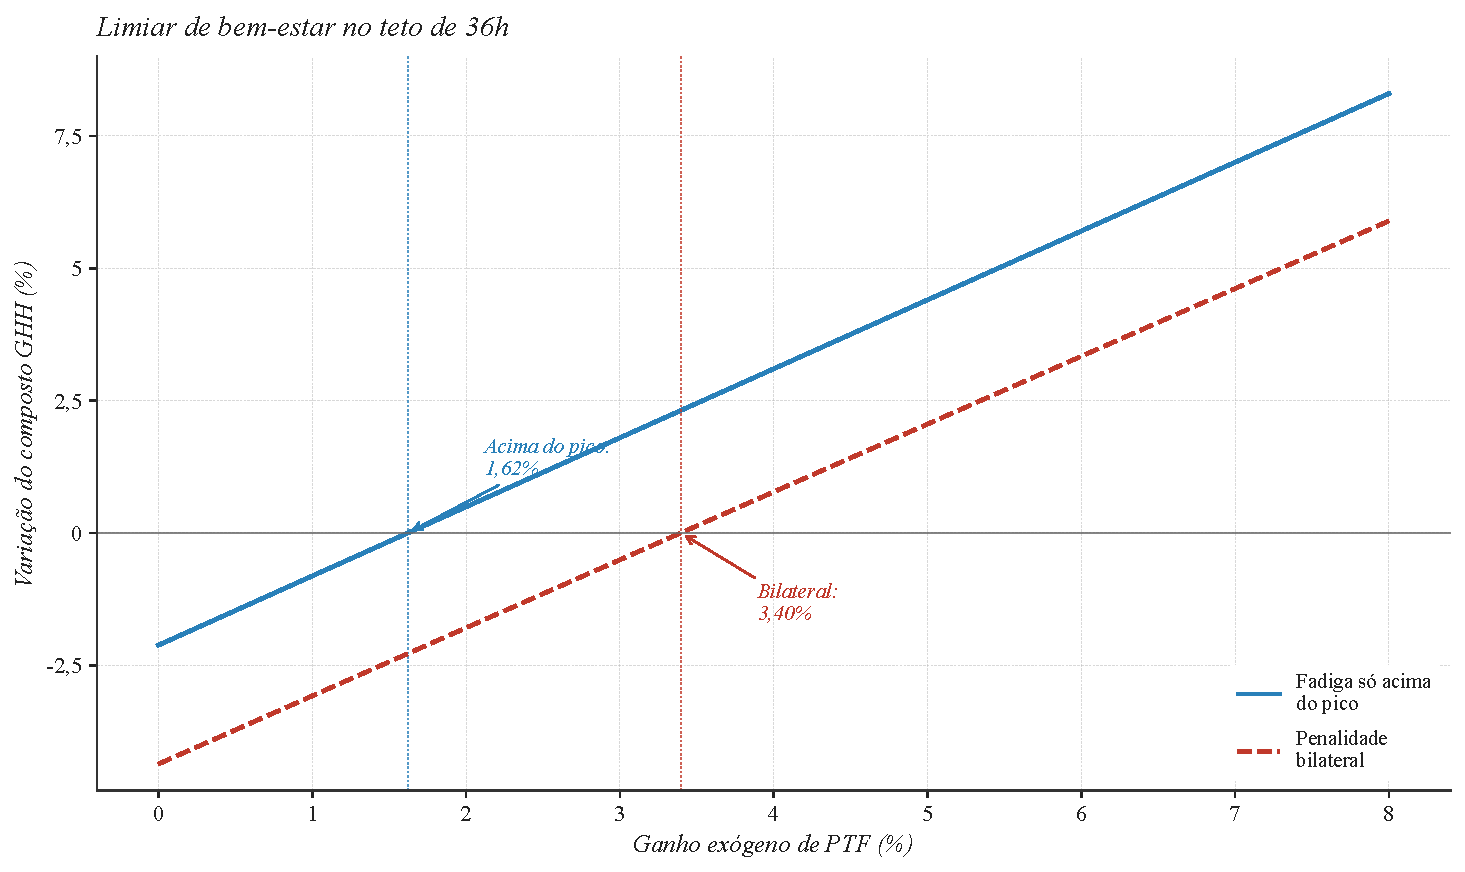
\includegraphics[width=0.95\textwidth]{generated/slide10c_welfare_threshold.pdf}
\caption{Limiar de bem-estar no teto de 36h}\label{fig:welfare_threshold}
\begin{minipage}{0.95\textwidth}\normalsize
\textit{Notas:} Variação percentual do composto GHH em função do ganho exógeno de PTF, relativamente à base formal limitada a 44h. Composição formal--informal reotimizada em cada avaliação, preservando ponte, cunhas e preferências iniciais. O indicador cruza zero em $3{,}39647\%$ de PTF na penalidade bilateral e em $1{,}62307\%$ sob fadiga só acima do pico. CE tem o mesmo numerador e o mesmo limiar, mas denominador diferente. Curvas e verificações estão em \path{generated/welfare_threshold.csv} e \path{generated/welfare_threshold_checks.json}.
\end{minipage}
\end{figure}
